\begin{document}
	
\newgeometry{left=2cm,right=2cm,bottom=1cm,top=1cm}
\pagestyle{empty}
\vfill
\vspace*{4cm}
\centerline{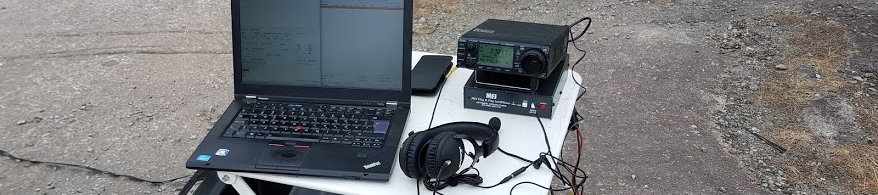
\includegraphics[width=\paperwidth]{logo/rubrikbild}}
\begin{flushright}
	\Huge{\bfseries{\TitleText}} \\[3mm]
	\Large{\bfseries{\SubtitleText}}
\end{flushright}

\vfill
	
Version: \DokVersion\ \hfill SMØUEI \hfill Datum: \DokumentDatum

\newpage

\newgeometry{top=3cm}

\pagestyle{fancy}
\lhead{\leftmark}
\rhead{
	\scriptsize
	\begin{tabular}{ll}
		\textbf{Version} & \textbf{Datum}\\
		\ \DokVersion & \DokumentDatum\\
	\end{tabular}
}

\chead{}

\lfoot{
	\scriptsize
	www.sm0uei.se
}

\cfoot{\scriptsize \thepage\ / \pageref{LastPage}}

\rfoot{\scriptsize
	anders@sikvall.se
}

\renewcommand{\footrulewidth}{0.2pt}

\widowpenalty=9999
\clubpenalty=9999

%	\setlength{\headsep}{1em}2

\cleardoublepage

%%% Innehållsförteckning
\tableofcontents

\newpage

\setlength{\parskip}{0.5em}
\setlength{\parindent}{0pt}

\section*{Förord}
	
Detta är den uppdaterade utgåvan för november 2023. Det var ett tag
sedan som jag ägnade mig åt det här alstret och det har kommit in lite
påpekanden om rättningar och att repeaterlistor med mera varit ganska
utdaterade. Det är förstås helt riktigt och jag har i skrivande stund
faktiskt försökt få in den färskaste informationen som finns från SSA.

Mycket har hänt sedan föregående information. Jag har flyttat från
Stockholm och har numera blivit SM5UEI men hänger fortfarande på
Kvarnbergets amatörradioklubb på torsdagskvällarna så där är det öppet
hus dessa dagar från kl. 19:00 när ni alla är välkomna att kika förbi.

Ändringar som skett sedan förra utgåvan:

\begin{itemize}[]
	\item Landsprefixdelen har kortats av och delats upp lite enligt 
	input från SMØMPV.
	\item Bandplanerna har setts över, bl.a. 60\,m-bandet i HF-delen 
	har lagts till då det saknades tidigare.
	\item Repeaterlistan uppdaterad med senaste data från SSA
	\item Gjort om några exempel-QSO enligt tips från SMØMPV
	\item En hel hoper med uppsnyggningar och förbättringar här och där.
\end{itemize}

Bidrag till handboken tas tacksamt mot men jag kommer bedöma ifall
materialet är lämpligt att ta med.  Hela materialet finns numera också
på Github om man vill gräva i det och fixa-dona, komma med 
förbättrings\-förslag och annat kul så finns den på följande länk:

\href{https://github.com/sikvall/rhb/}{https://github.com/sikvall/rhb}

Har ni en massa bra förslag på grejer som ni skulle vilja ha med i boken
så låt mig veta det där, det går också om ni vill arbeta in ändringar direkt
och skicka mig en s.k. "pull request" så kan jag kika på det. Det går också
att logga issues om man hittar fel.

Det går också hitta en massa annat radiorelaterat på min hemsida om ni är intresserade och där kan ni också normalt hitta radiohandboken som senaste version i PDF att ladda ner direkt.

\href{https://sikvall.se}{https://sikvall.se/}

Och kör radio där ute. Mobilt. Stabilt. Maritimt. Aeromobilt. Alltid med
stil.\\[4em]

Karlholm, \DokumentDatum\\
\textit{Täpp-Anders Sikvall\\
	SM5UEI}

\clearpage

\section*{Nyheter}

Vi börjar med det övergripande reglementet för radiotrafik när man inte har ett särskilt tillstånd för detta. Har man det står det i tillståndet vilka villkor som gäller för radiotrafiken men för de som nyttjar de så kallade licensfria banden så som PR-radio på 27 MHz, de gamla åkerikanalerna på 69 MHz, kortdistansradiobandet på 444 MHz, PMR-bandet på 446 MHz osv så finns reglerna samlade i en föreskrift från PTS som allmänt brukar kallas för ''Undantagsföreskriften''.

PTS har gjort en del uppdateringar av undantagsföreskriften som kan vara bra att kika igenom om det är något som berör de frekvenser du själv använder.

Vad gäller det senaste så kan man hitta mer information hos Post- och Telestyrelsen (PTS) på deras hemsida\footnote{\href{https://pts.se/radio/radiotillstand/undantag-fran-tillstandsplikt/}{https://pts.se/radio/radiotillstand/undantag-fran-tillstandsplikt/}} där det är den senaste versionen som gäller.

I föreskriften finns oerhört många radiofunktioner listade som inte är intressanta för oss men här står också vad som gäller i form av effekter och hur de olika banden eller kanalerna får nyttjas, i vilka sammanhang och ibland också till vilken grad. 

Det är en god idé att sätta sig in i detta och titta igenom detta ordentligt. Det kommer uppdateringar med jämna mellanrum och detta innebär också att det lönar sig att titta in då och då på PTS hemsida för att se vad som sker.

En intressant sak man kan läsa sig till här och som just nu är ute på remiss är faktiskt ett förslag till instegscertifikat för amatörradio!

\section*{Instegscertifikat för amatörradio}

För den som är seriöst radiointresserad så rekommenderar jag varmt att ta ett amatörradiocertifikat vilket ger tillgång till helt nya frekvensband och möjlighet att sända med högre effekter, kommunicera via satelliter, nytta det amatörernas egna IP-nät AMPRnet, sätta upp relästationer och mycket mycket mer. Här finns den bästa chansen också att i kris få tag i någon som kan hjälpa till. 

Nytt på den här fronten är ett förenklat instegscertifikat som PTS håller på att ta ställning till utformningen av. Det innebär ett förenklat prov vilket säkert hjälper en del som tycker att tekniken eller reglementet är för avancerat i det nuvarande certifikatet, men det kommer också innebära en del begränsningar. 

Dessa ser just nu ut att bli sådana att det blir en begränsad effekt, begränsningar i vilka band som får användas (endast band som är exklusiva för amatörradio, dvs inte 80 meter eller 70 cm som exempel) samt endast CE-märkt utrustning.

Mer information finns hos bland annat SSA och PTS.

\clearpage
	
